%! suppress = TooLargeSection
%! suppress = SentenceEndWithCapital
%! suppress = TooLargeSection
% Preamble
\documentclass[11pt]{PyRollDocs}
\usepackage{textcomp}
\usepackage{csquotes}
\usepackage{wasysym}


% Document
\begin{document}

    \title{Gripping analysis PyRolL Plugin}
    \author{Christoph Renzing}
    \date{\today}

    \maketitle

    This plugin provides a gripping analysis based on the geometrical conditions inside the roll gap.


    \section{Model approach}\label{sec:model-approach}

    In contrary to flat rolling, the gripping analysis for grooves has to be done locally.
    This is the case, since the roll radius varies and therefore the gripping condition has to be checked locally.
    To archive a local spatial resolution of the roll gap in the x-z plane, the groove and profile are discretized into so called \enquote{Gripping Elements}.
    Using the gripping elements, their local entry angle $\alpha_0$ and respected local roll radius $R_{W,l}$ are calculated.
    Through this information, the geometric gripping analysis can be evaluated according to equation~\ref{eq:gripping-condition}.
    Figure~\ref{fig:roll-gap-forces} shows the force conditions in the roll gap during gripping.

    \begin{figure}
        \centering
        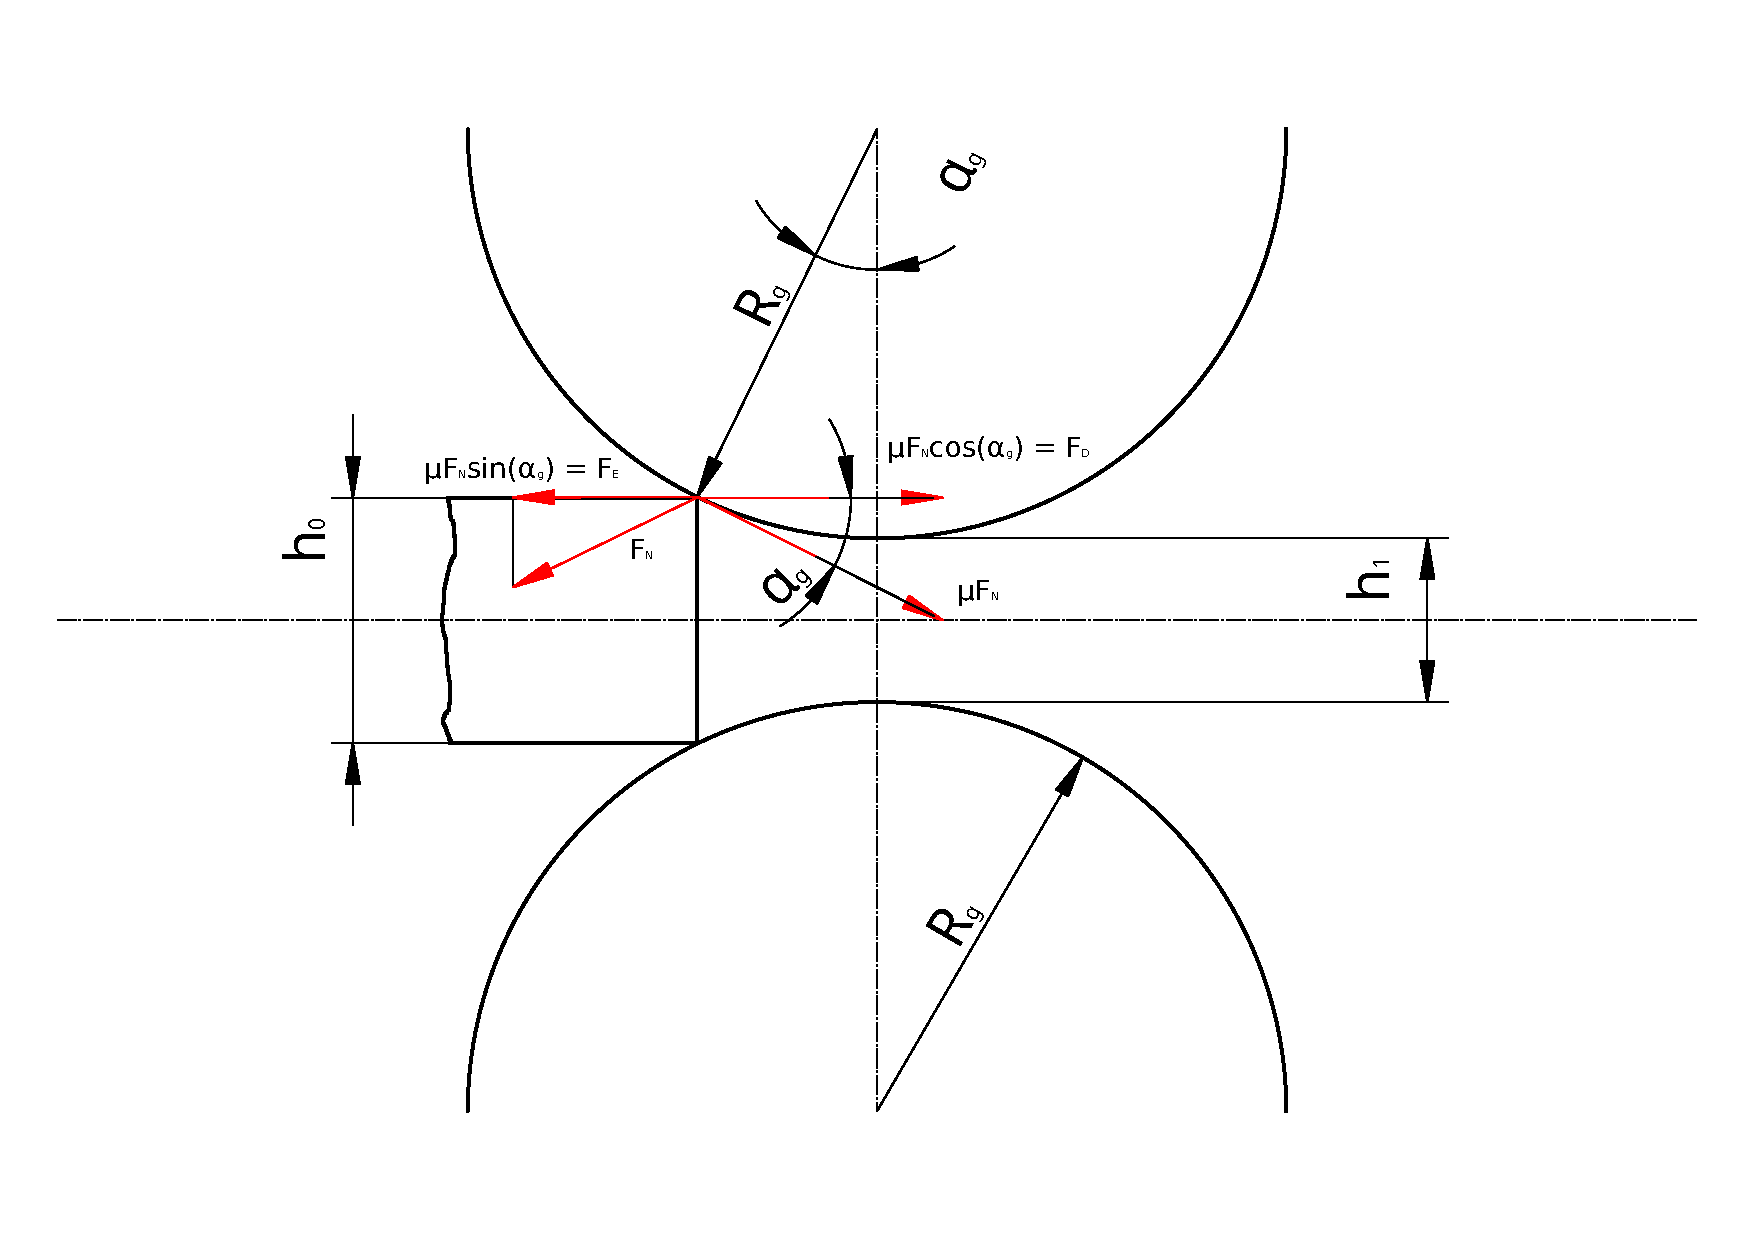
\includegraphics[width=.5\textwidth]{img/gripping-forces}
        \caption{Force acting at the point of gripping in the roll gap}
        \label{fig:roll-gap-forces}
    \end{figure}

    \newpage

    Due to friction, the normal force $F_N$ generates a tangential force $F_T$, see equation~\ref{eq:tangential-force}.

    \begin{equation}
        F_T = \mu F_N
        \label{eq:tangential-force}
    \end{equation}

    In order for the incoming profile to be drawn into the roll gap, the forces drawing the material into the roll gap ($F_D$),
    must be greater than the ejecting force ($F_E$), so that equation~\ref{eq:forces-while-gripping} applies.

    \begin{equation}
        F_D = \mu F_N \cos\left( \alpha_{0} \right) \geq F_E = \mu F_N \sin\left( \alpha_{0}  \right)
        \label{eq:forces-while-gripping}
    \end{equation}

    From this the grip condition can be determined, see equation~\ref{eq:gripping-condition}.

    \begin{equation}
        \mu \geq \tan\left( \alpha_{0} \right)
        \label{eq:gripping-condition}
    \end{equation}

    The second assumption used for this case, is that the initial contact point between profile and roll happens at a distance which is represented by the contact length.

    \begin{equation}
        L_{d, l} = \sqrt{R_{W, l} \Delta h_{max} - \frac{\Delta h_{max}^2}{4}}
        \label{eq:contact-length-gripping}
    \end{equation}

    This is valid only for the case, that the material of both the roll and the profile behaves purely plastic.
    Using this assumption, the rolling angle $\alpha$ can be calculated using trigonometric relations.

    \begin{equation}
        \alpha_{0, l} = \arcsin\left( \frac{L_{d, l}}{R_{W, l}} \right)
        \label{eq:gripping-angle}
    \end{equation}


    \section{Usage instructions}\label{sec:usage-instructions}

    The plugin can be loaded under the name \texttt{pyroll\_gripping\_analysis}.
    The plugin defines the hooks \lsto

    \begin{table}[h]
        \centering
        \caption{Hooks specified by this plugin.}
        \label{tab:hookspecs}
        \begin{tabular}{ll}
            \toprule
            Hook name                            & Meaning                                                            \\
            \midrule
            \texttt{gripping\_elements}          & Center points of the gripping elements                             \\
            \texttt{gripping\_elements\_heights} & Heights of the gripping elements according to the incoming profile \\
            \texttt{passed\_gripping\_condition} & Boolean resulting in True or False                                 \\
            \bottomrule
        \end{tabular}
    \end{table}


\end{document}